\section{Introduction}

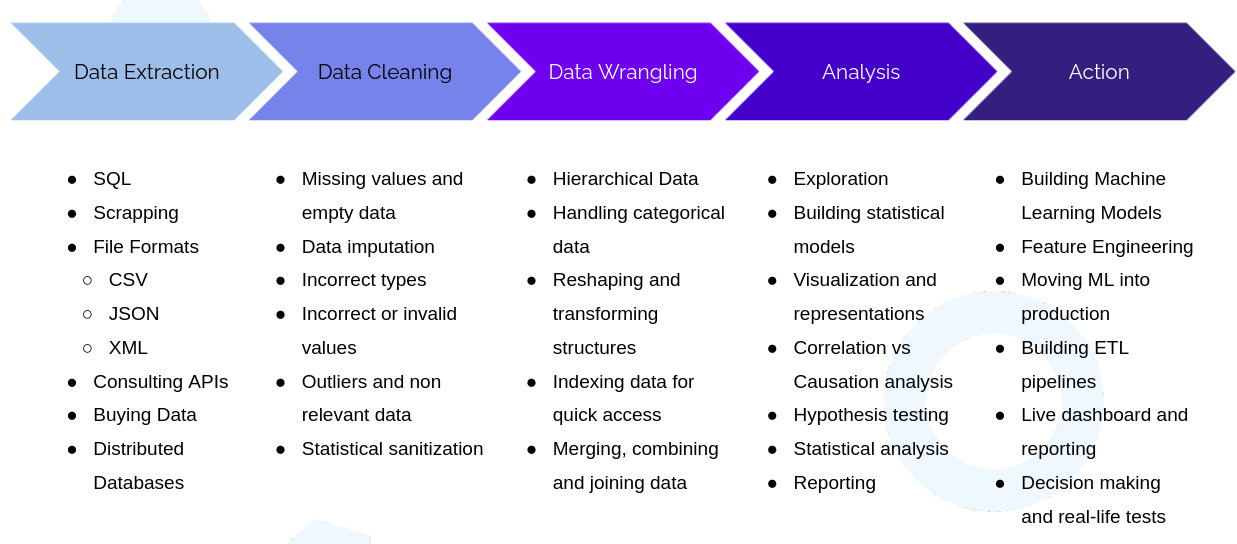
\includegraphics[scale=0.2]{pictures/data_analysis_process.png}

Useful libraries:
\begin{itemize}
  \item pandas
  \item numpy
  \item matplotlib
  \item scipy
\end{itemize}



\section{Read/Write files}

\begin{minted}{python}
    df = pd.read_csv(csv_file_name)
    df.to_csv('file_name.csv')
\end{minted}


\section{DataFrame}

\begin{minted}{python}
    # Create dataframe
    df = pd.DataFrame({
        'col_1': value.index,
        'col_2': value,
        ...
    })

    # Analysis
    df.info()           # info about dataset
    df.description()    # statistical info about dataset
    df.columns()        # dataframe columns

    # Indexing
    x = df.column_title                 # single column target
    x = df[['culumn_title_1'], ...]     # multiple columns targets

    
\end{minted}

